\subsection{Population Genetics}

Population genetics is the study of relationships between populations and between species, the study of evolution. Before technology allowed us to study the genetic material, scientists had to rely on morphological data and archeological findings. Since the genetic material is inherited from generation to generation it holds the molecular history of all living things so it provides another very nice tool for doing population genetics. When studying the genetic material, or genome, in any sexually reproducing organism we'll find that all species are more or less related by similarity but each individual has its own unique combination of variants in the form of structural variations, single nucleotide variations (SNV) and copy number aberrations. There are many known and probably unknown evolutionary mechanisms controlling the processes that give rise to these variations. We will not go into detail of how this machinery works in this essay, just outline some terminology that will be used later on.\\

% Dubbelkolla denna referens av population!
% Detta stycke ska även handla mer om hundar.
% Kolla upp sympatric populations
We define a \textbf{population} as a group of organisms of one species, living in one area \cite{fundamental}. In this work we have focused on dogs so the definition of populations is not perfect. Since we have different breeds that have been conceived in one area and then perhaps moved to another, a population of dogs can both be regional or a breed. We define a gene as a union of genomic sequences encoding a coherent set of potentially overlapping protein products \cite{gerstein07}. An \textbf{allele} is defined as a variant of a gene, a \textbf{haplotype} is a combination of alleles. A \textbf{gene pool} is all alleles of a gene in a population.\\


One of the basic assumptions when talking about origin of species by looking at molecular data, is that \textbf{the sub population with the biggest genetic diversity is closest related to the anscestral population.} This assumption is based on the idea that a species has a number of founder individuals who holds all the added variations inherited from the ancestral species. When sub populations migrate they carry with them a subset of the variations, also this population have had the longest time to develop new variants from molecular evolutionary events. We can think of this like a Venn diagram where all variation of the ancestral population is symbolized by a big circle, when subpopulations emigrate they bring a part of the whole variation with them.\\

\begin{figure}[ht]
	\centering
		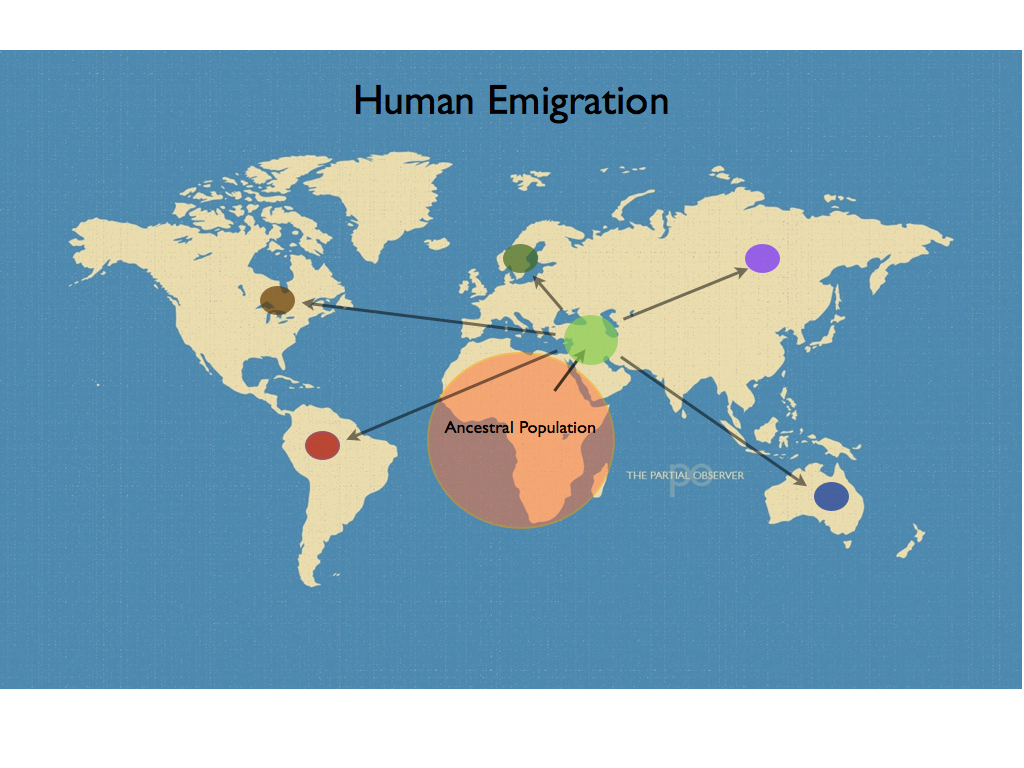
\includegraphics[width=0.6\textwidth]{../pictures/Single_origin_1.jpg}
	\caption{Human migration events: The picture describes how the populations have spread out from Africa about 125000-65000 years ago \cite{born_in_africa}. Circles represent the genetic diversity found in the populations.}
	\label{fig:human_migrations}
\end{figure}


The most well studied example of this is humans, here the Out Of Africa Theory was founded before genetic material was accessible. The theory was based on archeological findings from around the world and the idea is that all humans originate in Africa and then migrated to the rest of the world, as illustrated in figure \ref{fig:human_migrations}. These finding have then been confirmed over and over again when studying the genetic material of human populations. Since humans is a relatively young species we tend to see, as in figure \ref{fig:human_migrations} and \ref{fig:single_origin}, that almost all variants from any population can be found in the ancestral population, which is the African population south of Sahara.\\


\begin{figure}[ht]
	\centering
		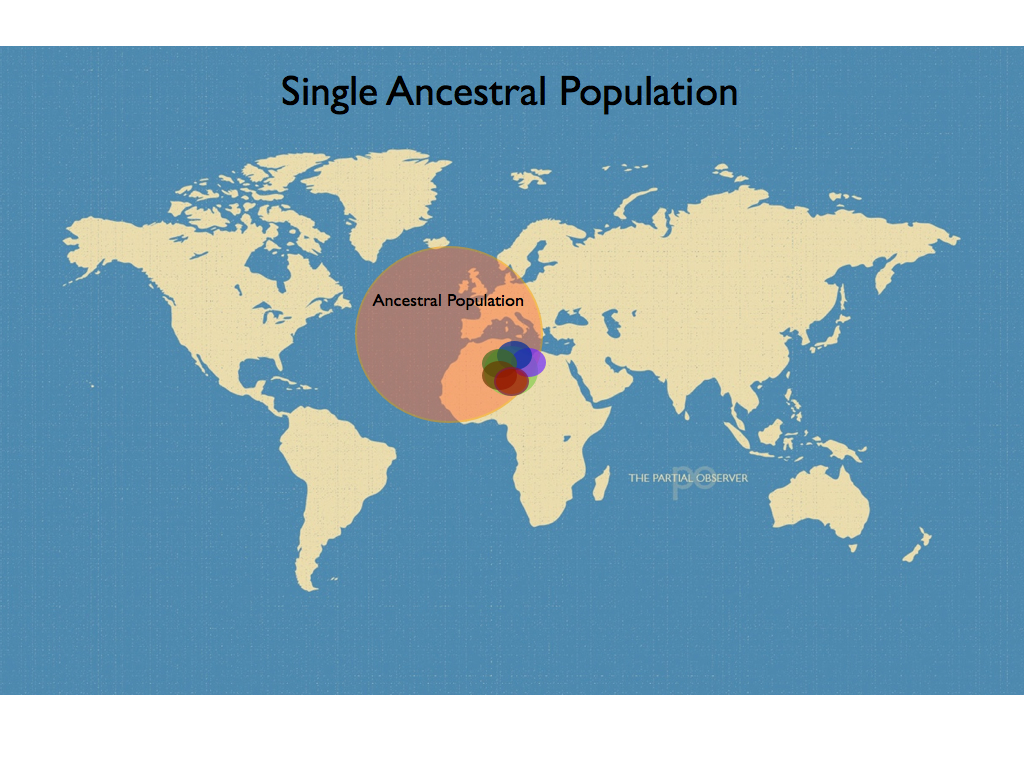
\includegraphics[width=0.6\textwidth]{../pictures/Single_origin_2.jpg}
	\caption{Human migration events: In the picture each circle represent the genetic diversity collected from populations all around the world. When compared to the suspected founder population , the African population south of Sahara here  represented by the the big circle, we find that all genetic variations from the populations can be found in the founder population.}
	\label{fig:single_origin}
\end{figure}


% Kolla upp Y-chromosome som markör, kanske ska vara "en del y-kromosomen" av denna eller liknande.

When trying to infer population history from molecular data one has until recently been limited to using so called genetic markers. This means that a fairly small and easy accessible part of genetic material is revealed in individuals from as many populations possible, this limitation was due to lack of technology and cost of sequencing. Two well used markers has been \textbf{mitochondrial DNA (mtDNA)} and parts of the \textbf{Y-chromosome}. mtDNA is a small chromosome apart from the nuclear DNA that we usually think of as the genome, some of the advantages of mtDNA as a genetic marker is that they are abundant in cells and inherited only on the \textbf{maternal} side, they only recombinate with other almost identical mtDNA resulting in minimal structural variation and has a high mutation rate \cite{cann87}.\\ 

The Y-chromosome is inherited only on the \textbf{paternal} side and does also not recombine (except for a small part that recombines with the X-chromosome) \cite{underhill07}. The Y-chromosome has been examined in several human \cite{jobling03,kayser01} and animal population studies \cite{ginja08,ling10}. The more genetic markers that are used the more information we can get of the history of evolution. When studying a single genetic marker only, we can more or less get the big picture but if we want to know more specific things like time for bottleneck events, migration and so on we need to have more markers or, most preferable, whole genome data \cite{stoneking11}.

\subsubsection{Origin of Dogs}

Morphological, behavioral and molecular data all agree that dogs originates from wolf \cite{clutton-brock95,vila97,wayne93} but the geographical origin of dogs is still debated. The first ideas of origin are based on archeological findings that point to multiple breeding events in South West Asia and Europe\cite{clutton-brock95,dayan94}.\\
There are several problems with making assumptions from archeological data, among others there will be bias to where the most excavations have been located and it can be hard to make a difference between species when there is only a limited amount of material, in our case dogs and wolves.\\
The archeological findings haved been complemented with genetic information, and the ruling hypotheses are currently that dogs originate from either single or multiple wolf populations in Europe \cite{benecke87,verginelli05}, Middle East \cite{gray10,vonholdt10} and/or South East Asia \cite{savo02, pang09, ding11}.\\

In contrast to what picture \ref{fig:human_migrations} and \ref{fig:single_origin} show, if we had multiple origins and collected genetic informaton from different populations we would expect to see something like in figure \ref{fig:multiple_origin} and \ref{fig:no_common_variation}.\\

\begin{figure}[ht]
	\centering
		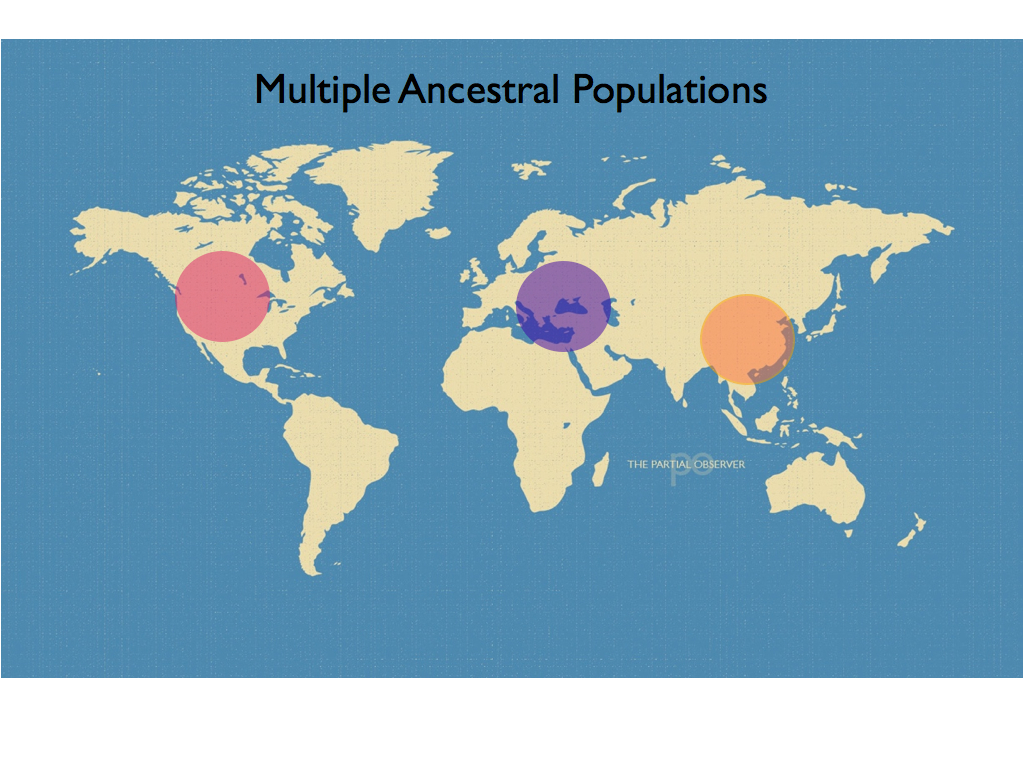
\includegraphics[width=0.5\textwidth]{../pictures/Multiple_ancestors_1.jpg}
	\caption{Multiple Ancestral Populations: The circles represent genetic pools of different populations.}
	\label{fig:multiple_origin}
\end{figure}

\begin{figure}[ht]
	\centering
		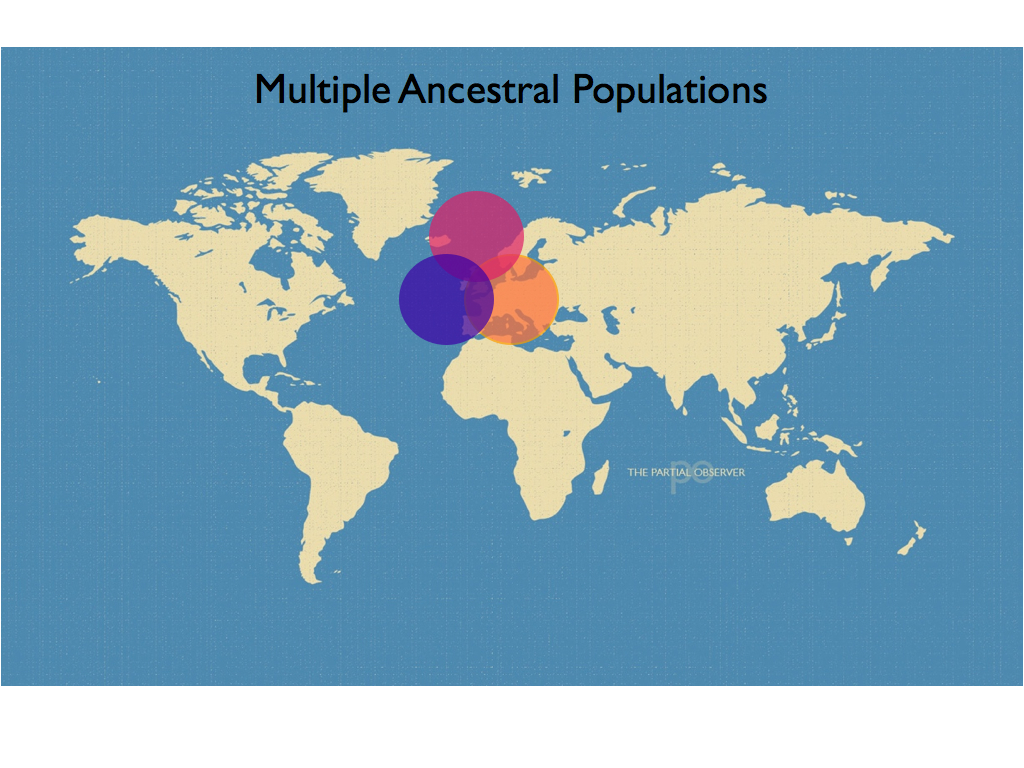
\includegraphics[width=0.5\textwidth]{../pictures/Multiple_ancestors_2.jpg}
	\caption{Multiple Ancestral Populations: If we where to compare the genetic information for populations of a species with multiple origin, we would expect to find large variations between the populations.}
	\label{fig:no_common_variation}
\end{figure}

After looking at genetic variation in a small number of dog breeds for a forensic study, Peter Savolainen and co workers started to suspect a different view of dog origin \cite{savo97}. They could see that, even in a small data set, dogs from the asian breeds had a greater genetic diversity than dogs from other breeds.\\

In 2002, Savolainen et.{ }al.{ }published an article \cite{savo02} where they proposed a single East Asian origin for the domestic dog about 15,000 years ago, based on variation in parts of mtDNA. In a more extensive mtDNA study published 2009 \cite{pang09} 10 major haplotypes where found in dog populations from all around the world. Among these the only population to include all haplotypes was in South East Asia south of Yangtze River, implying a single origin in this region. The results where confirmed again in 2011 \cite{ding11} when variation in the Y-chromosome was studied.
These findings might seem unquestionable but there is still an ongoing discussion of how many times and where dogs where domesticated.\\ 

In this work we have tried to develop a method to genotype a small hypervariable region of genomic DNA with errors created during the sequencing process. If we succeed in genotyping these individuals, we can see how genetic diversity of this marker correlate with the earlier findings described above. We expect to see the biggest diversity among the wolves and the second biggest among dogs sampled south of Yangtze River.  



